\section{Diskretizacija problema}

Funkcije $\mathbsf{A}\mathbf{(x)}$, $\mathbf{v(x)}$, $\mathbf{u(x)}$ in $\mathbf{f(x)}$ v variacijski izjavi \eqref{eq:LsfemVariationalStatement} so bile do te točke popolnoma svobodne. Dopuščali smo vse možne oblike odvisnosti, ki jih lahko napnemo nad domeno $\Omega$. Če želimo z reševanjem splošnega problema \eqref{eq:compactPDE} nadaljevati, moramo svobodo odvisnosti omejiti. Poljubno funkcijo $\mathbf{v(x)}$ na domeni $\Omega$ aproksimiramo s sestavljanko N \textbf{vozliščnih funkcij} $\mathbf{\Phi}_i$:
\begin{equation}
    \mathbf{v(x)} = \sum_{i = 1}^N v_i  \mkern1mu \mathbf{\Phi}_i \ .
\end{equation}
Za primer vzemimo kvadratno domeno s krajevnim vektorjem $\bm{\chi} = \{\xi,\eta\} \in [-3,\mkern2mu 3\mkern1mu] \mkern-1mu \times \mkern-1mu [-3,\mkern2mu 3\mkern1mu]$ in nanjo postavimo pravokotno mrežo $N = 16$ vozlišč (slika \ref{fig:regionAndNodeFunctions}a). Vsakemu vozlišču pripadata vozliščna funkcija $\mathbf{\Phi}_i(\bm\chi)$ in \textbf{vozliščna vrednost} $v_i\mkern2mu$, ki predstavlja višino vozliščne funkcije v tej točki. Skozi oči \texttt{FI} je $\ket{\Phi_i}$ eden izmed baznih vektorjev v razvoju vektorja $\ket{v}$, $v_i$ pa pripadajoča komponenta. Ploskvice, ki sestavljajo mrežo, imenujemo elementi.

\begin{figure}[ht]
    \begin{subfigure}[b]{0.42\textwidth}
        \centering
        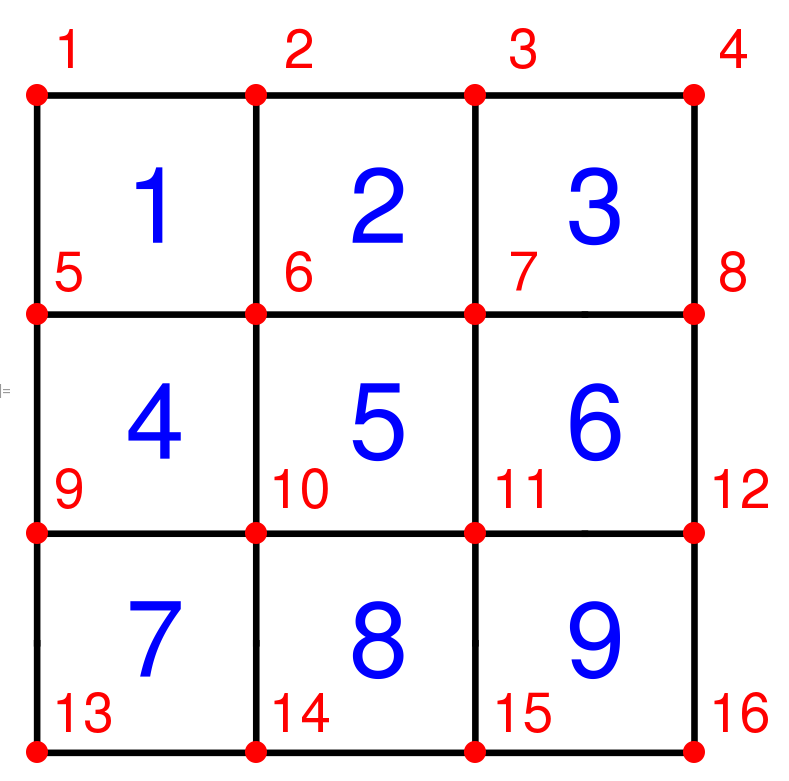
\includegraphics[height=67mm]{Slike/undeformedRegion.png}
        \vspace{6mm}
        \caption{}
    \end{subfigure}
    \begin{subfigure}[b]{0.55\textwidth}
        \centering
        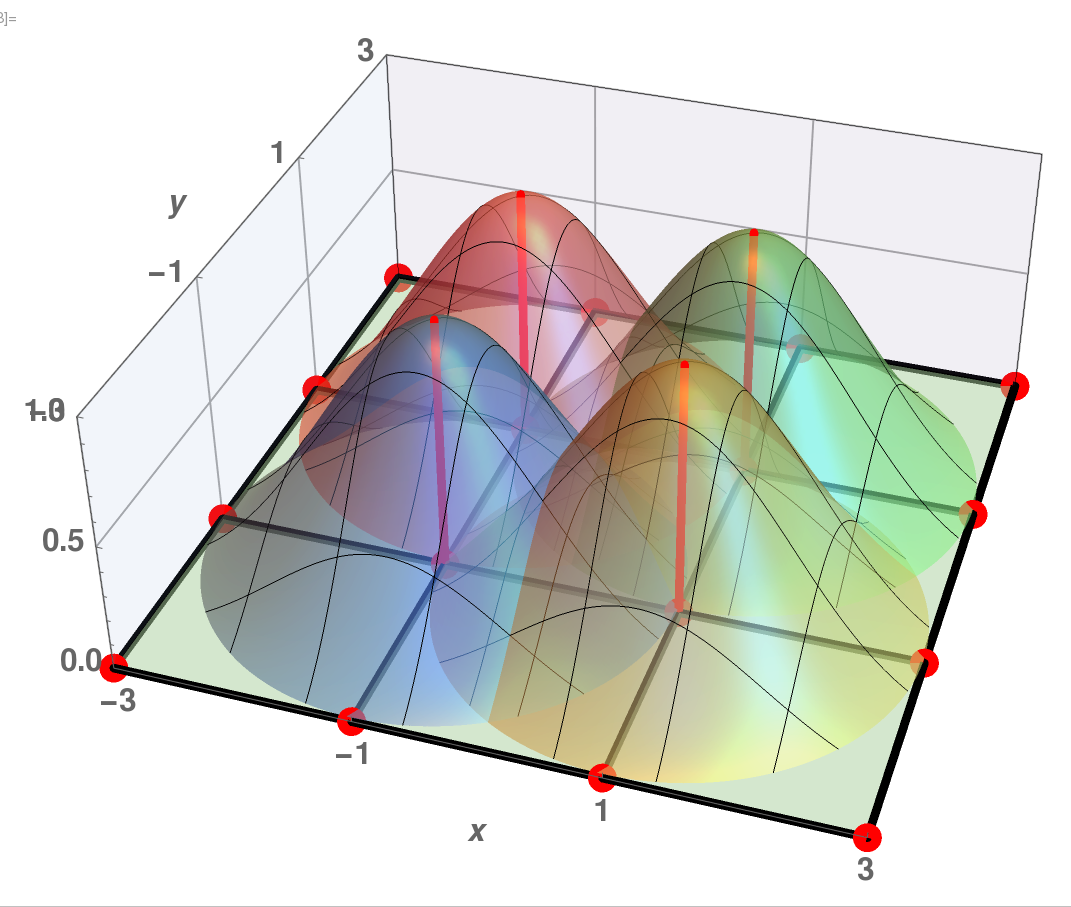
\includegraphics[width=0.94\textwidth]{Slike/undeformedNodeFs.png}
        \caption{}
    \end{subfigure}
    \caption{(a) pravokotna domena s šestnajstimi vozlišči (rdeča) in devetimi elementi (modra) ter (b) nad vozlišči napete vozliščne funkcije.}
    \label{fig:regionAndNodeFunctions}
\end{figure}

\begin{figure}[ht]
    \begin{subfigure}[b]{0.48\textwidth}
        \centering
        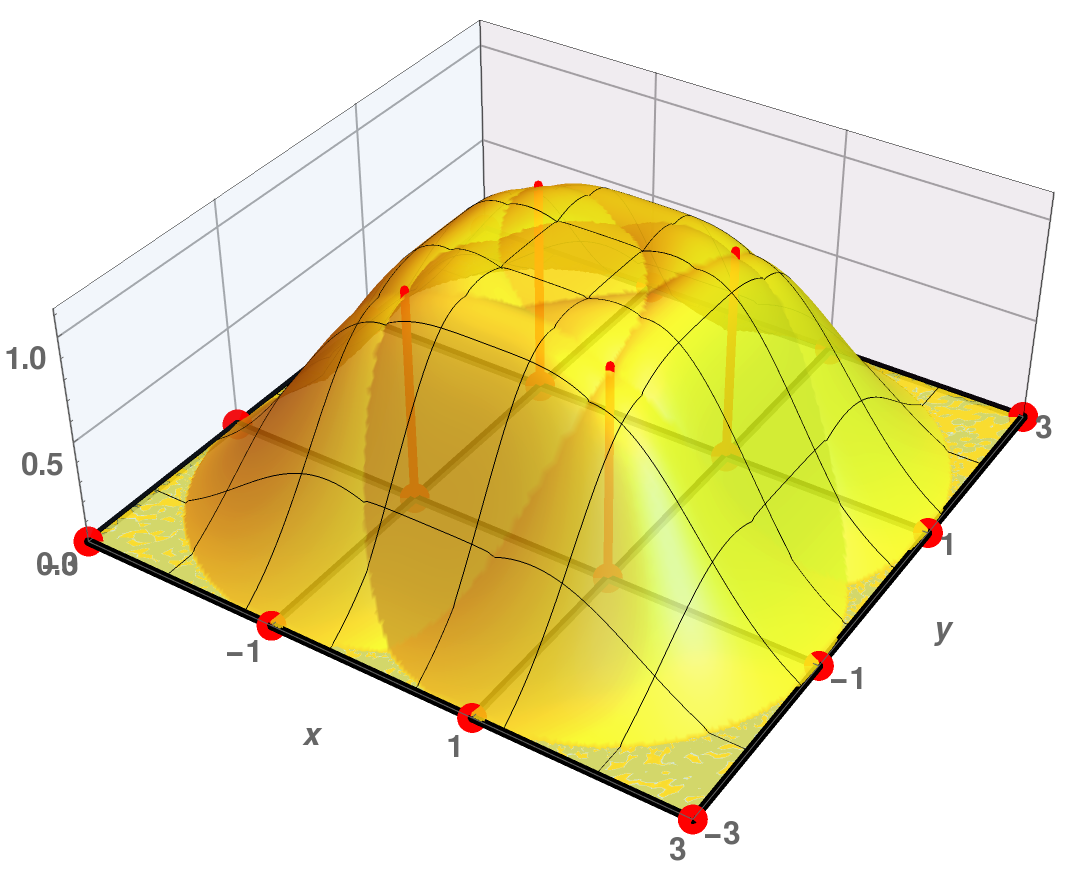
\includegraphics[width=0.94\textwidth]{Slike/sumOfNodeFs.png}
        \vspace{6mm}
        \caption{}
    \end{subfigure}
    \begin{subfigure}[b]{0.48\textwidth}
        \centering
        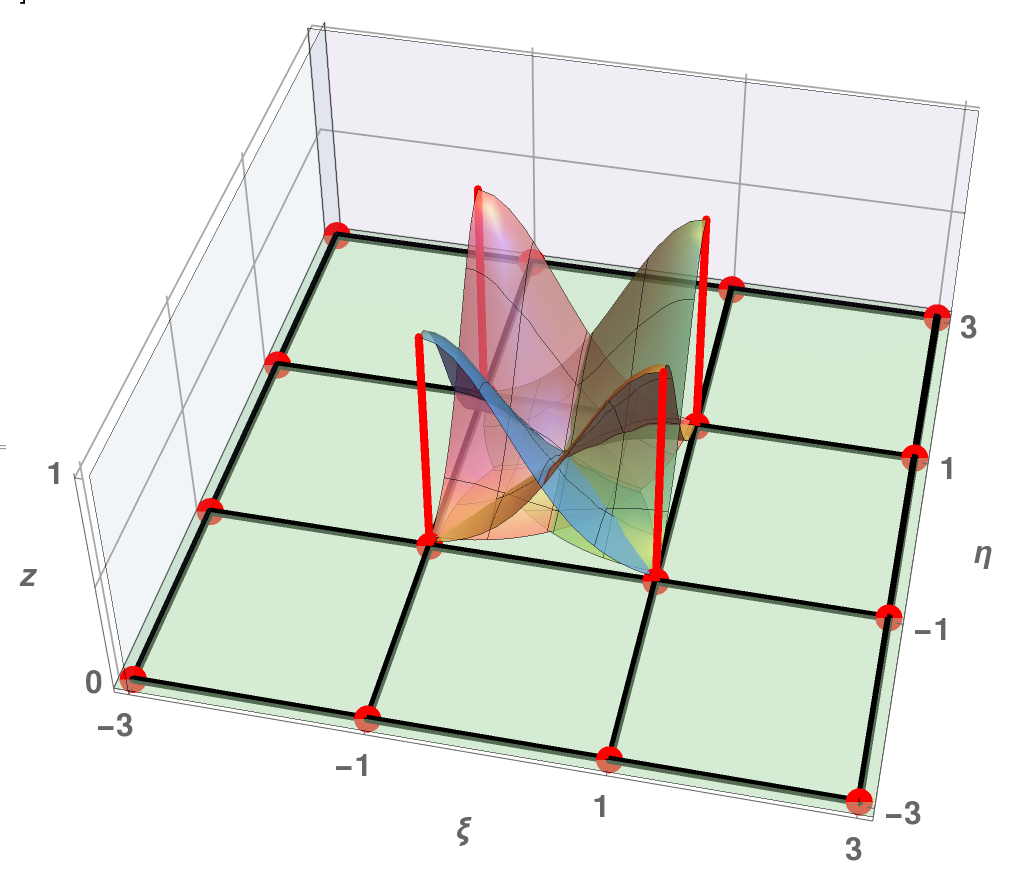
\includegraphics[width=0.94\textwidth]{Slike/undeformedShapeFsFar.png}
        \caption{}
    \end{subfigure}
    \caption{(a) pravokotna domena s šestnajstimi vozlišči (rdeča) in devetimi elementi (modra) ter (b) nad vozlišči napete vozliščne funkcije.}
    \label{fig:sumAndShapeFunctions}
\end{figure}

še vedno  Z natančno analitično izpeljavo se prebijemo do izjave \eqref{eq:LsfemVariationalStatement}, od tod dalje pa moramo iskanje funkcije $\mathbf{u(x)}$ z neskončno prostostnimi stopnjami poenostaviti v iskanje funkcije s končnim številom prostostnih stopenj $N$. 

V jeziku funkcionalne analize (\texttt{FI}) pravimo, da smo omejili funkcijski prostor.

nadaljujemo z diskretizacijo problema, to je, pretvorbo na sistem $N$ algebrajskih enačb. Ta korak je enak pri vseh različicah \texttt{FEM}. Funkcije na domeni $\Omega$ imajo neskončno štveilo prostostnih stopenj. 
\begin{equation}
    u_i(\mathbf{x}) = \sum_{a = 1}^N \Phi^{a0} u^{a0}_i
\end{equation}

Potem omejimo Diskretizacija problema 

Galerkin, Najmanših kvadratov \cite{JiangB-LSFEM}
Basic lemma of variational principles: Temeljni lema variacijskih načel.